\documentclass[../main.tex]{subfiles}

\begin{document}

\subsection{Motivación}

Más del 80\% de los datos que se manejan están sin estructura en la forma de texto en lenguaje natural (libros, informes, noticias, artículos de investigación, mensajes de redes sociales y páginas webs).

En años recientes ha habido un auge en la minería de textos y el procesamiento de lenguaje natural.

La minería de textos es la confluencia de procesamiento de lenguaje natural, minerías de datos, aprendizaje automático y estadística usados para extraer conocimientos de textos no estructurados.

La popularización de Internet y las tecnologías de comunicación móviles ha atraído la atención en la minería de textos. Campo de aplicación como la minería de opiniones y análisis de datos médicos y financieros.

\begin{figure}[h]
	\centering
	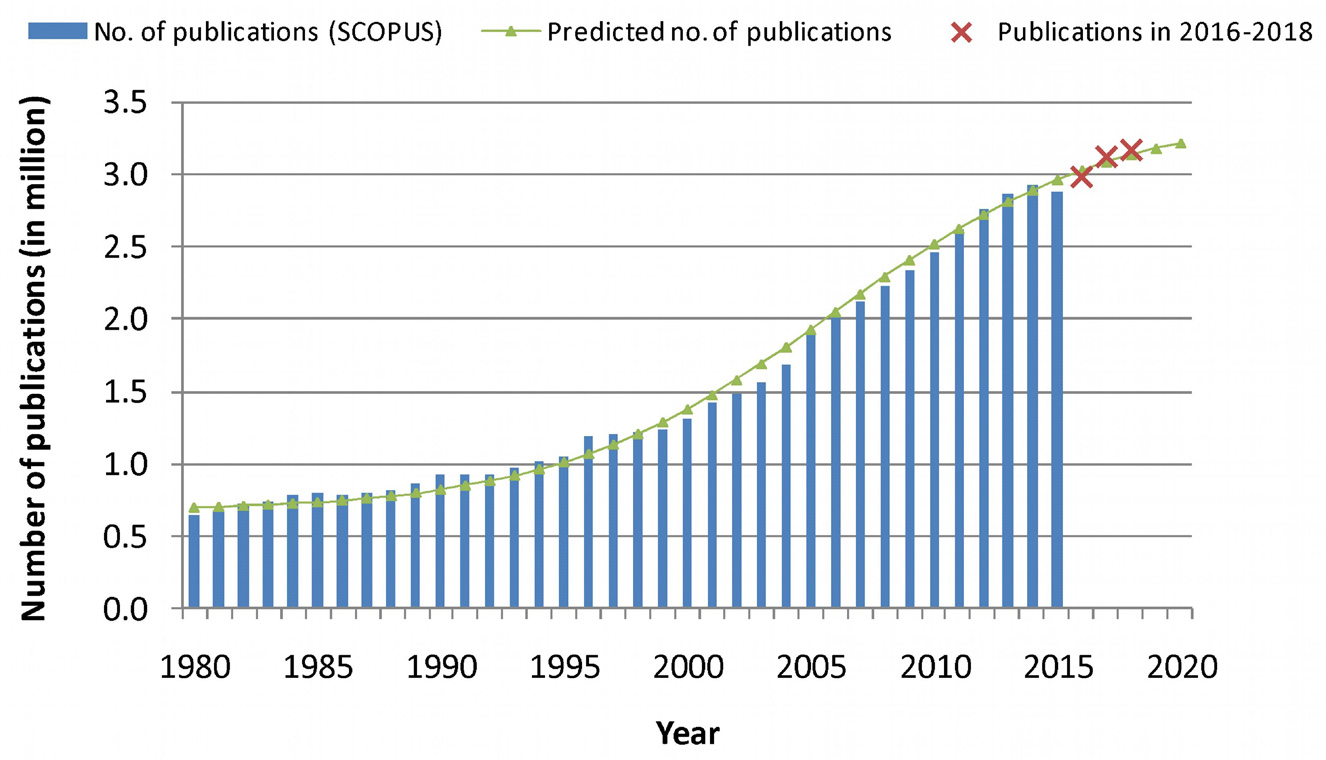
\includegraphics[width=0.7\textwidth]{../images/publications-per-year.jpg}
	\caption{Publicaciones por año. \cite{to2020rise}}
	\label{fig:publications-year}
\end{figure}

Los artículos de investigación son empleados en el mundo académico. La cantidad de publicaciones que se realizan anualmente van incrementándose cada año (Figura \ref{fig:publications-year}). Organizar o buscar un artículo en concreto para su posterior lectura requiere un tiempo valioso. Este se puede reducir si previamente se extraen los metadatos de cada uno de los artículos. De este modo se pueden filtrar los resultados y así obtener información útil.


\subsection{Objetivos}

El objetivo del proyecto es buscar metainformación de los artículos de investigación (papers) en formato PDF.

\begin{itemize}
	\item El planteamiento preliminar para alcanzar el objetivo es utilizar NLP (procesamiento de lenguaje natural).
	Con esta herramienta se analiza el texto y se intenta encontrar algún patrón que encaje en alguno de los metadatos a buscar.
	\item Se buscarán las palabras más repetidas del texto por ser las más significativas.
	\item De entre los metadatos a extraer se encuentran el título y el autor.
	\item También se debe contabilizar el número de páginas, tablas y figuras del artículo.
\end{itemize}

\subsection{Estructura}

Este documento está dividido en cinco partes.

En primer lugar se encuentra esta introducción donde se establecen las bases del proyecto.
A continuación, en la segunda parte, se explican los conceptos que se utilizan a lo largo de esta memoria.
Le sigue la sección «Herramientas» donde se enumeran las distintas aplicaciones y librerías que se han empleado para la realización del proyecto.
Posteriormente, la sección cuarta, «Desarrollo», describe los pasos necesarios para realizar el proyecto.
Por último, en «Resultados» se muestran las gráficas y comentarios sobre los resultados obtenidos.

Además, se incluye un apéndice con los pasos a seguir para la instalación de Anaconda en Linux.

\end{document}
